\documentclass{article}
\usepackage[utf8]{inputenc} %кодировка
\usepackage[T2A]{fontenc}
\usepackage[english,russian]{babel} %русификатор 
\usepackage{mathtools} %библиотека матеши
\usepackage[left=1cm,right=1cm,top=2cm,bottom=2cm,bindingoffset=0cm]{geometry} %изменение отступов на листе
\usepackage{amsmath}
\usepackage{graphicx} %библиотека для графики и картинок
\graphicspath{}
\DeclareGraphicsExtensions{.pdf,.png,.jpg}
\usepackage{subcaption}
\usepackage{pgfplots}
\usepackage{amssymb}
\usepackage{physics}
\title{\LaTeX}
\date{}
\author{}

\begin{document}
\maketitle
\section{Введение в интеграл ФНП}
1. \textbf{Определение Интегрируемой Функциональной Функции}: \\
   Начните с определения функционала (интегрируемой функциональной функции), которую вы хотите интегрировать. Обычно эта функциональная функция зависит от некоторой переменной, например, функции $f(x)$, где $x$ - независимая переменная в ФНП.

2. \textbf{Выбор Диапазона Интегрирования}: \\
   Укажите диапазон интегрирования. В случае определенного интеграла это будет интервал или множество значений переменной, на котором вы хотите произвести интегрирование.

3. \textbf{Разбиение Интервала}: \\
   Если ваша функциональная функция зависит от переменной $x$, разбейте интервал интегрирования на подынтервалы. Это может потребоваться для численного вычисления интеграла.

4. \textbf{Вычисление Интеграла}: \\
   Сам интеграл в ФНП будет представлен в виде:
   \[
   \int_{a}^{b} F[f(x)] d\mu(x),
   \]
   где $F[f(x)]$ - функционал, зависящий от функции $f(x)$, $d\mu(x)$ - мера в ФНП. Вычисление этого интеграла может потребовать применения специальных методов, в зависимости от задачи и меры в ФНП.

5. \textbf{Вычисление Значения}: \\
   Вычислите значение интеграла, используя выбранный метод интегрирования или численные методы, если это необходимо.

6. \textbf{Интерпретация Результата}: \\
   Проанализируйте полученный результат с учетом контекста задачи. Понимание значения интеграла важно для той области математики или физики, в которой он применяется.

7. \textbf{Подведение Итогов}: \\
   Заключите ваш конспект, подводя итоги построения и вычисления определенного интеграла в ФНП и подчеркивая его важность в соответствующей области знаний.

\section{Двойной интеграл}
Двойной интеграл - это интеграл от функции двух переменных по области в двумерном пространстве. Вот некоторые из основных свойств двойного интеграла:

   1. **Линейность**: Двойный интеграл линеен, что означает, что сумма или разность интегралов функций равна интегралу суммы или разности этих функций. Формально: 
      \[
      \iint_D [f(x, y) + g(x, y)] \, dA = \iint_D f(x, y) \, dA + \iint_D g(x, y) \, dA
      \]
   
   2. **Аддитивность**: Если область интегрирования разбивается на несколько непересекающихся подобластей, то двойный интеграл по всей области равен сумме двойных интегралов по каждой из подобластей. Формально:
      \[
      \iint_D f(x, y) \, dA = \sum_{i} \iint_{D_i} f(x, y) \, dA
      \]
      где $D$ - область интегрирования, $D_i$ - подобласти.
   
   3. **Инвариантность относительно порядка интегрирования**: Порядок интегрирования по переменным $x$ и $y$ может быть изменен без изменения результата:
      \[
      \iint_D f(x, y) \, dA = \iint_D f(y, x) \, dA
      \]
   
   4. **Изменение переменных**: Можно сделать замену переменных в двойном интеграле, чтобы упростить интегрирование. Например, можно использовать полярные координаты для интегрирования функций с радиальной симметрией.
   
   5. **Свойство неравенства**: Если $f(x, y) \leq g(x, y)$ для всех точек в области интегрирования $D$, то:
      \[
      \iint_D f(x, y) \, dA \leq \iint_D g(x, y) \, dA
      \]
   
   6. **Свойство монотонности**: Если $f(x, y) \leq g(x, y)$ для всех точек в области интегрирования $D$, и $D$ имеет площадь, то:
      \[
      \iint_D f(x, y) \, dA \leq \iint_D g(x, y) \, dA
      \]
   
   7. **Симметрия**: Если функция $f(x, y)$ симметрична относительно центра координат или имеет другие виды симметрии, это может упростить вычисление двойного интеграла.
   
   Эти свойства полезны при решении различных математических и физических задач, в которых требуется вычисление двойных интегралов.
\\ \\
Теорема о вычислении двойного интеграла, также известная как теорема о смене порядка интегрирования, утверждает, что значение двойного интеграла не изменяется при изменении порядка интегрирования. Это важное свойство, которое позволяет упростить вычисления во многих задачах. Формально эта теорема может быть сформулирована следующим образом:

Пусть функция $f(x, y)$ непрерывна на замкнутой области $D$ в плоскости $xy$, где $D$ определена конечными интегралами:

\[
D = \{(x, y) \mid a \leq x \leq b, g_1(x) \leq y \leq g_2(x)\},
\]

где $a \leq x \leq b$, и функции $g_1(x)$ и $g_2(x)$ также непрерывны на $[a, b]$. Тогда двойной интеграл функции $f(x, y)$ по области $D$ может быть вычислен в следующих двух формах:

1. **По вертикальным полосам**: Сначала интегрируем по переменной $y$, а затем по переменной $x$:
   
   \[
   \iint_D f(x, y) \, dA = \int_{a}^{b} \int_{g_1(x)}^{g_2(x)} f(x, y) \, dy \, dx
   \]

2. **По горизонтальным полосам**: Сначала интегрируем по переменной $x$, а затем по переменной $y$:
   \[
   \iint_D f(x, y) \, dA = \int_{a}^{b} \int_{g_1(x)}^{g_2(x)} f(x, y) \, dy \, dx
   \]

где $c$ и $d$ - это значения, соответствующие области $D$ по оси $y$, и функции $h_1(y)$ и $h_2(y)$ также непрерывны на $[c, d]$.

Таким образом, теорема о вычислении двойного интеграла позволяет выбирать наиболее удобный порядок интегрирования в зависимости от задачи, что может значительно упростить вычисления.
\\ \\
\textbf{Двойной интеграл в криволинейных координатах}
\begin{center}
    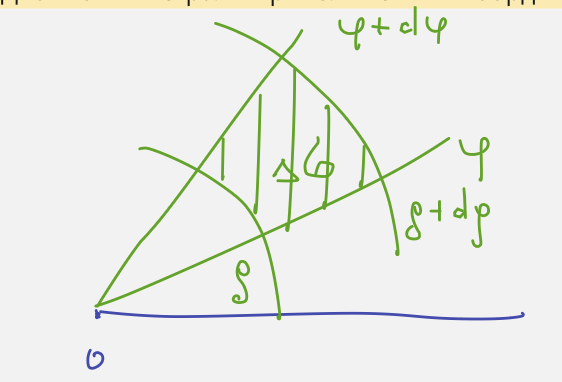
\includegraphics[width=.3\textwidth]{123} 
\end{center}
\begin{equation*}
    \Delta \sigma = \frac{d\phi}{2\pi}(\pi (\rho + d\rho)^2-\pi\rho ^2)
\end{equation*}

\begin{equation*}
    d \sigma = \rho d\phi d\rho
\end{equation*}
\begin{equation*}
    \iint_{D}f(x;y)dxdy=\iint_{D'}f(\rho cos\phi;\rho cos\phi)\rho d\phi d\rho
\end{equation*}
\begin{center}
    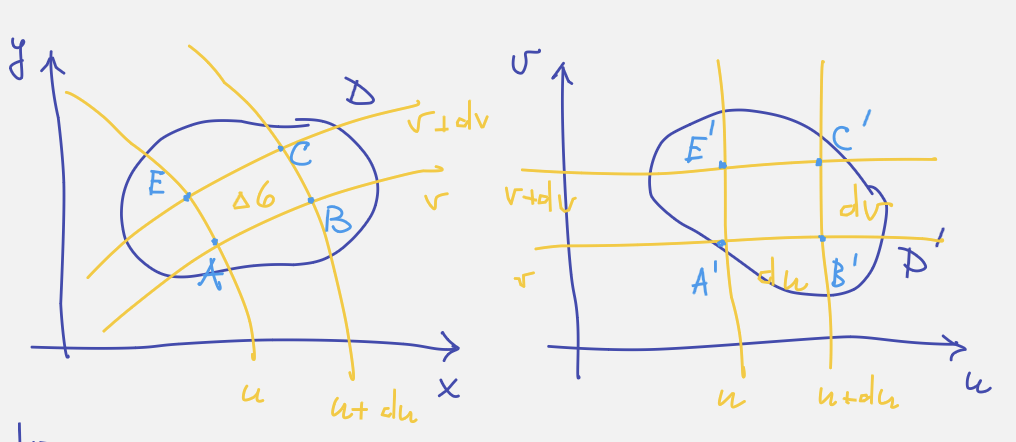
\includegraphics[width=.3\textwidth]{krivo.png}
\end{center}
Предположим, у вас есть двойной интеграл в декартовых координатах (x, y):

\[I = \iint_D f(x, y) \, dA,\]

и вы хотите выполнить переменные преобразования, чтобы перейти к новым координатам (u, v):

\[\begin{cases} u = u(x, y) \\ v = v(x, y) \end{cases}\]

Тогда вы можете выразить элемент площади dA в новых координатах как:
\begin{equation*}
    A(x_1; y_1):\ x_1 = x(u;v),\ y_1 = y(u;v)
\end{equation*}
\begin{equation*}
    B(x_2; y_2):\ x_2 = x(u+du;v),\ y_2 = y(u+du;v)
\end{equation*}
\begin{equation*}
    C(x_3; y_3):\ x_3 = x(u+du;v+dv),\ y_3 = y(u+du;v+dv)
\end{equation*}
\begin{equation*}
    E(x_4; y_4):\ x_4 = x(u;v+dv),\ y_4 = y(u;v+dv)
\end{equation*}
\\


1) Криволин. параллелограмм приблизим прямыми

2) Пренебрежём бесконечно малыми порядка 2 и выше
\begin{equation*}
    A'(x';y')\ \ \ x'_1 = x(u, v);\ y'_1 = y(u, v)
\end{equation*}
\begin{equation*}
    B'(x';y')\ \ \ x'_2 = x(u, v) + \pdv{x}{u}du;\ y'_2 = y(u, v) + \pdv{y}{u}du
\end{equation*}
\begin{equation*}
    C'(x';y')\ \ \ x'_3 = x(u, v) + \pdv{x}{u}du + \pdv{x}{v}dv;\ y'_3 = y(u, v) + \pdv{y}{u}du + \pdv{y}{v}dv;
\end{equation*}
\begin{equation*}
    E'(x';y')\ \ \ x'_4 = x(u, v) + \pdv{x}{v}dv;\ y'_4 = y(u, v) + \pdv{y}{v}dv
\end{equation*}
\\ \\
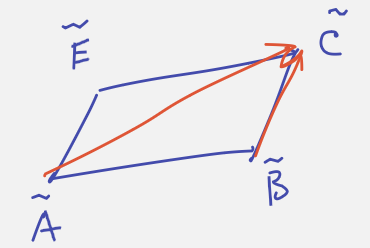
\includegraphics[width=.3\textwidth]{paral.png} 
\begin{equation*}
    S_{abce}= 2 S_{abc} = 2\frac{1}{2}|BC'\ x \ AC'| = 
    \left|\left|\begin{matrix}
        i\ j\ k\\
        x'_3-x_2'\ y'_3-y_2'\ 0\\
        x'_3-x_1'\ y'_3-y_1'\ 0
    \end{matrix}\right|\right|= 
    \left|\left|\begin{matrix}
        \pdv{x}{u}\ \pdv{x}{v}\\
        \pdv{y}{u}\ \pdv{y}{v}
    \end{matrix}\right|\right|dvdu
\end{equation*}
Модуль Якобиана
\begin{equation*}
    dA =  
    \left|\left|\begin{matrix}
        \pdv{x}{u}\ \pdv{x}{v}\\
        \pdv{y}{u}\ \pdv{y}{v}
    \end{matrix}\right|\right|dvdu
\end{equation*}
\section{Тройной интеграл}
\begin{equation*}
    \mathcal{V} \in \mathbb{R}:\text{ огранич замкнут пов-ю S тело}
\end{equation*}
\begin{equation*}
    f(x;y;z) \text{ непрерывна в $\mathcal{V}(на границе S тоже)$}
\end{equation*}
Схема интеграла

1) n элементарных объёмов $\Delta \mathcal{V}_i\ i=1...n$

2) $P_i(x_i;y_i;z_i)\in \Delta\mathcal{V}_i$

$f(P_i)=f(x_i;y_i;z_i)\ \ f(P_i)\cdot \Delta \mathcal{V}_i$ \ \ \ $f(P_i)\cdot \Delta \mathcal{V}_i = \Delta G_i$

3) $G_n = \sum_{i=1}^{n}\Delta G_i= \sum_{i=1}^{n}f(P_i)\Delta \mathcal{V}_i$
4)$\lambda -> 0$ = $max(diam\Delta \mathcal{V}_i)$

$\lim_{n->\inf;\lambda->0}G_n = \lim_{n->\inf;\lambda->0}\sum_{i=1}^{n}\Delta G_i= \lim_{n->\inf;\lambda->0}\sum_{i=1}^{n}f(P_i)\Delta \mathcal{V}_i$

$G=\iiint_{\mathcal{V}}dG=\iiint_{\mathcal{V}}f(x;y;z)d\mathcal{V} = \iiint_{\mathcal{V}}f(x;y;z)dxdydz$
\section{Криволиненйный интеграл}
\textbf{ПЕРВЫЙ РОД}
\begin{center}
    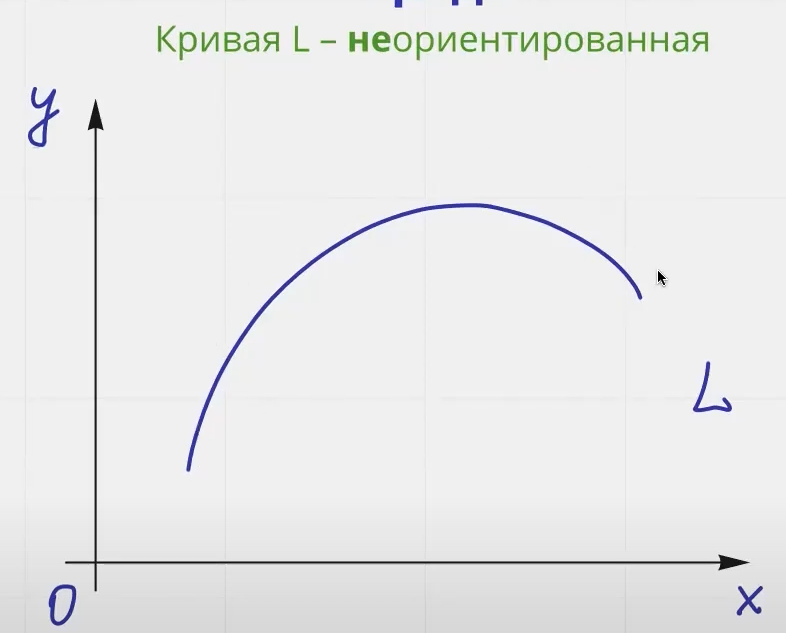
\includegraphics[width=.3\textwidth]{rod1.png}
\end{center}
\begin{equation*}
    z = f(x,y)
\end{equation*}
\begin{center}
    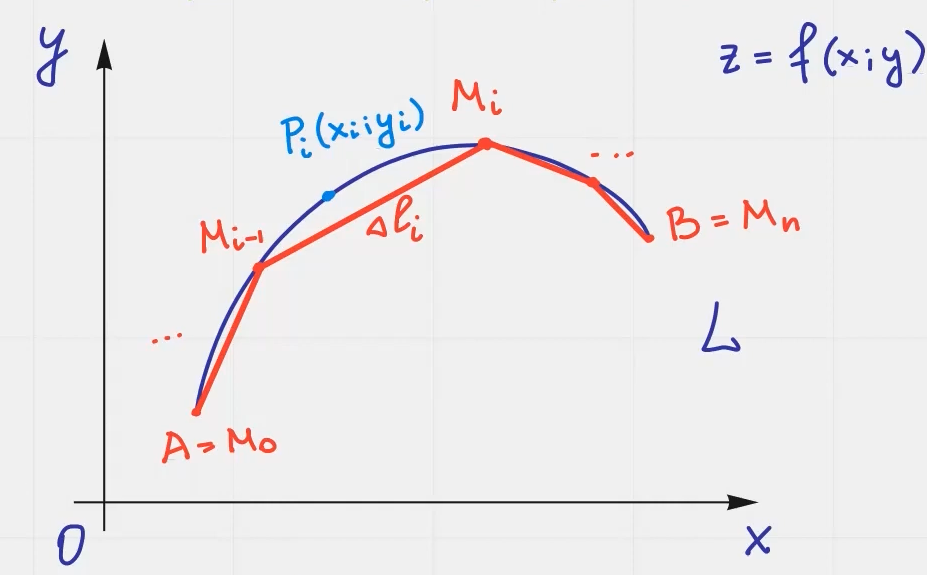
\includegraphics[width=.3\textwidth]{krivo12.png}
\end{center}
\begin{equation*}
    \lim_{n->\inf; \lambda->0}\sum_{i=1}^{n}f(x_i; y_i)\Delta l_i = \int_{L}^{}f(x;y)dl
\end{equation*}
Криволинейный интеграл 1 рода по длине дуги. Для непрерывных функций.

Свойства:

1) Линейность: $\int(a) = a\int$

2) Аддитивность: $\int(+) = \int+\int$

3) Оценка: мин - мин плостность умнож на длину и аналогично для макс 

4) Среднее значение

5) Не заданно направление, без разницы в какую сторону идти по длине при подсчёте чего-либо. Независимость от ориентированности кривой от интегрирования.
\begin{equation*}
    \int_{AB}^{} f(x;y)dl = \int_{BA}^{} f(x;y)dl
\end{equation*}
\textbf{Вычисление}

Параметрически задана:
\begin{equation*}
    L:
    \begin{cases}
        x=x(t)\\
        y=y(t)
    \end{cases},t\in[ t;t_2]
\end{equation*}

\begin{equation*}
    \int_{L}^{}f(x;y)dl = \int_{t_1}^{t_2}f(x(t);y(t))\sqrt{x'^2(t)+y'^2(t)}dt\ \ \ t_1<t_2
\end{equation*}
\begin{equation*}
    \Delta l_i = \sqrt[]{\Delta x_i^2+\Delta y_i^2}=\left|\Delta x_i = x'(\overline{t}_i)\Delta t_i; \Delta y_i = y'(\overline{t'}_i)\Delta t_i\right| = 
    \sqrt{x'^2(\overline{t}_i)+y'^2(\overline{t'}_i)}\abs{\Delta t_i}
\end{equation*}
\begin{equation*}
    dl = \sqrt{x'^2(t)+y'^2(t)}dt
\end{equation*}

Задана явно:
\begin{equation*}
    L: y=y(x),\ x\in [a;b]
\end{equation*}
\begin{equation*}
    dl = \sqrt{1+y'^2(x)}dx;\ \ \ \int_{a}^{b}f(x; y(x))\sqrt{1+y'^2(x)}dx
\end{equation*}

Задана полярно:
\begin{equation*}
    L: \rho = \rho(\phi),\ \ \ \phi \in [\phi_1;\phi_2]
\end{equation*}
\begin{equation*}
    dl = \sqrt{\rho(\phi)^2+\rho'(\phi)^2}d\phi; \ \ \ \int_{\phi_1}^{\phi_2}f(\rho(\phi) cos\phi;\rho(\phi)sin\phi)\cdot \sqrt{\rho(\phi)^2+\rho'(\phi)^2}d\phi
\end{equation*}

\textbf{ВТОРОЙ РОД}

Кривая ориентированная
\begin{center}
    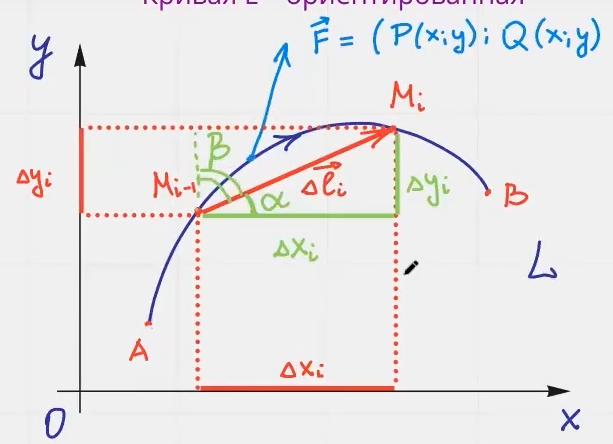
\includegraphics[width=.3\textwidth]{krivo2.png} 
\end{center}

\begin{equation*}
    \overline{F} = (P;Q)
\end{equation*}
\begin{equation*}
    \Delta \overline{l}_i = (\Delta x_i; \Delta y_i)
\end{equation*}
\begin{equation*}
    \Delta A_i = \overline{F}\cdot \Delta \overline{l}_i = P\Delta x_i+Q\Delta y_i
\end{equation*}
\begin{equation*}
    \int_{L}^{}dA = \int_{L}^{}\overline{F}\cdot d \overline{l} = \int_{L}^{}Pdx+Qdy
\end{equation*}
Интеграл соответствует, если функция непрерывна 


Свойства:

1) Линейность: $\int(a) = a\int$

2) Аддитивность: $\int(+) = \int+\int$

3) Оценка: мин - мин плостность умнож на длину и аналогично для макс 

4) Среднее значение

5) Заданно направление. Зависимость от ориентированности кривой от интегрирования. Смена знака при смене обхода

\begin{equation*}
    \int_{AB}^{}\overline{F}d\overline{l} = -\int_{BA}^{}\overline{F}d\overline{l}
\end{equation*}

6) Связь кривол интеграла 1 рода и 2 рода
\begin{equation*}
    d\overline{l} = (cos\alpha\cdot dl; cos\beta\cdot dl; )=\tau^o dl
\end{equation*}
\begin{equation*}
    \int_{L}^{}\overline{F}\cdot d\overline{l} = \int_{L}^{}\overline{F}\cdot \tau\cdot dl = \int_{L}^{}F_{||}\cdot dl
\end{equation*}
\begin{equation*}
    \int_{L}^{}Pdx+Qdy = \int_{L}^{}(Pcos\alpha + Q cos\beta)dl
\end{equation*}
\textbf{Вычисление}

Явно:
\begin{equation*}
    y= y(x),\ x\in [a,b]
\end{equation*}
\begin{equation*}
    \int_{L}^{}Pdx+Qdy = +\  or\ - \int_{a}^{b}P(x;y(x))dx+Q(x;y(x))y'(x)dx
\end{equation*}
\\
\begin{equation*}
    x= x(y),\ x\in [c,d]
\end{equation*}
\begin{equation*}
    \int_{L}^{} Pdx +Qdy = +\ or\ -\int_{c}^{d}P(x(y);y)x'(y)dy +Q(x(y);y)dy
\end{equation*}
Параметрически:
\begin{equation*}
    L: \begin{cases}
        x=x(t)\\
        y=y(t)
    \end{cases}, t\in[t_1;t_2]
\end{equation*}
\begin{equation*}
    \int_{L}^{}Pdx+Qdy = +\ or \ - \int_{t_1}^{t_2}P(x(y);y)x'(y)dy +Q(x;y(x))y'(x)dx
\end{equation*}

\section{Поверхностный интеграл}
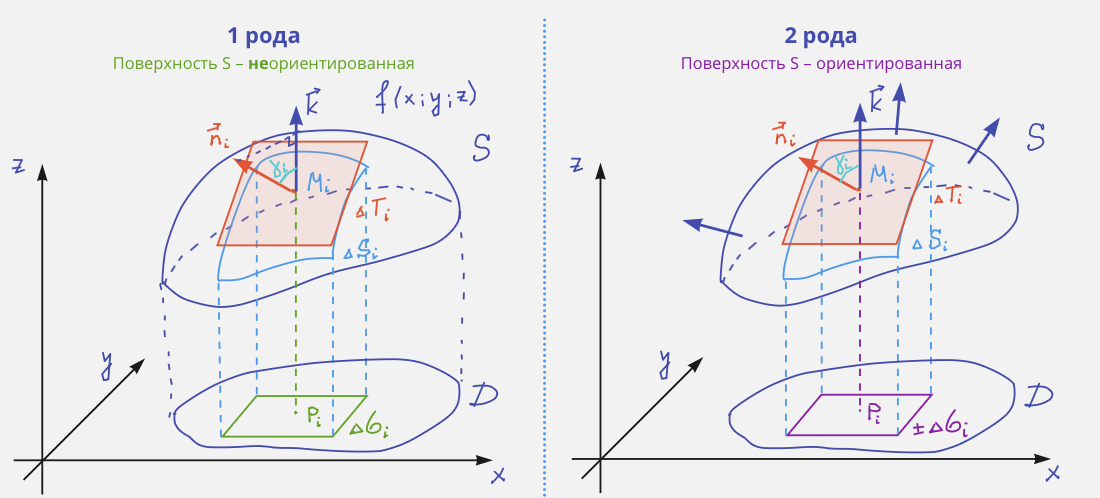
\includegraphics[width=.8\textwidth]{butilka.png}
\\ 
\textbf{1 род}
\\
Поверхностный интеграл
\begin{equation*}
    \lim_{n->\infty; \lambda->0}\sum_{k=1}^{n}f(x_i;y_i;z_i)\Delta S_i =\iint_S f(x;y;z)dS 
\end{equation*}
Свойства:

1) Линейность

2) Аддитивность

3) Теорема об оценке: $m_{min} \cdot S \leq \iint_S fdS\leq M_{max}\cdot S$, m - min f(), M - max f()

4) т.о среднем: соответствует $M'\in S: f(M')\cdot S = \iint_S fdS$; M' - среднее значение f на поверх S

5) Независимость от ориентации поверхность.
\\
Вычисление:

\begin{equation*}
    \Delta \sigma_i = \Delta T_i \cdot cos\gamma_i
\end{equation*}

\begin{equation*}
    d\sigma = dxdy = dS\cdot cos\gamma
\end{equation*}

\begin{equation*}
    cos\gamma = \frac{|\overline{n}\cdot \overline{k}|}{|\overline{n}|\cdot |\overline{k}|}
\end{equation*}
\begin{equation*}
    F(x;y;z) = 0 
\end{equation*}
\begin{equation*}
    \overline{n} = gradF = (F'_x; F'_y; F'_z); \ \ k =(0;0;1)
\end{equation*}
\begin{equation*}
    dS = \frac{1}{|F'_z|}\sqrt{F'^2_x+F'^2_y+F'^2_z}dxdy
\end{equation*}
\begin{equation*}
    \iint_S f(x;y;z)dS = \iint_{D_{xy}}f(x;y;z(x;y))\frac{\sqrt{F'^2_x+F'^2_y+F'^2_z}}{|F'^2_z|}dxdy
\end{equation*}
\begin{equation*}
    z = z(x;y);\ \ z - z(x;y) = 0; \ \ \iint_S f(x;y;z)dS = \iint_{D_{xy}}f(x;y;z(x;y))\sqrt{z'^2_x+z'^2_y+1}dxdy
\end{equation*}
\\
Приложение 

Площадь
\begin{equation*}
    S = \iint_S dS 
\end{equation*}

\begin{equation*}
    G_S = \iint_S f(x;y;z)dS 
\end{equation*}
\\ 
\textbf{2 род}
\\
Поверхностный интгерал 2 рода (по проекции поверхности)
\begin{equation*}
    \lim_{n->\infty; \lambda-> 0}\sum_{k=1}^{n}f(x_k;y_k;y_k)\Delta \sigma_k = \iint_S F(x;y;z)d\sigma
\end{equation*}

Свойства:

1) Линейность

2) Аддитивность

3) Теорема об оценке: $m_{min} \cdot S \leq \iint_S fdS\leq M_{max}\cdot S$, m - min f(), M - max f()

4) т.о среднем: соответствует $M'\in S: f(M')\cdot S = \iint_S fdS$; M' - среднее значение f на поверх S

5) Зависимость от ориентации поверхности.

6) Связь с 1 рода 

\begin{equation*}
    \iint_S Rdxdy + \iint_S P dy dz +\iint_S Q dzdx = \iint_S Pdydz + Qdzdx +Rdxdy = \iint_S (Pcos\alpha dS + Qcos\beta dS + Rcos\gamma)dS
\end{equation*}
\\
Вычисление:
\begin{equation*}
    \iint_S F(x;y;z)dxdy = +(if\ n\ and \ k \ ugol\ osrt)-(if\ n\ and\ k\  ugol\ tupoy)\iint_{D_{xy}}R(x;y;z(x;y))dxdy 
\end{equation*}
\section{Формулы Стокса и Остроградского-Гаусса}
Рассмотрим $S - $ гладкая поверхность в трёхмере\\
$L - $ контр, огранич $S$\\
$P, Q, R - $ непрерывна дифф на L и на S.\\

\begin{equation*}
    \overline{F} = (P;Q;R)
\end{equation*}
\begin{equation*}
    \ointop_{L}\overline{F}d\overline{l} = \ointop_{L}dA
\end{equation*}
Циркуляция поля F вдоль L\\
\textbf{Стокс}
\begin{equation*}
    \ointop_L Pdx + Qdx + Rdx  = \iint_S (\pdv{R}{y}-\pdv{Q}{z})dydz+(\pdv{P}{z}-\pdv{R}{x})dzdx+(\pdv{Q}{x}-\pdv{P}{y})dxdy
\end{equation*}
\textbf{Остроградский-Гаусс}\\
T - тело в $\mathbb{R}^2$, S - граница тела Т, т.е. замкн пов-ть (гладкая)\\
P,Q,R 
\begin{equation*}
    \iint_S Pdydz +Qdzdx+ Rdxdy = \iiint_T (\pdv{P}{x}+\pdv{Q}{y}+\pdv{R}{z})dxdydz
\end{equation*}
$\overline{F} = (P;Q;R),\ d\overline{S} = (dydz;dzdx;dxdy)$
\begin{equation*}
    \iint_{S^+} \overline{F}d\overline{S} = \iiint_T div\overline{F}dv
\end{equation*}
% \begin{equation*}
    
% \end{equation*}
% \section{}
% 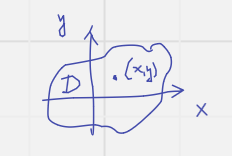
\includegraphics[width=.3\textwidth]{1.1} 
\end{document}
